\documentclass[11pt]{article}
\usepackage[margin=0.84in]{geometry}
\usepackage{amsmath,amssymb,amsthm,graphicx,microtype}
\usepackage[hidelinks]{hyperref}
\setlength{\parindent}{0pt}
\setlength{\parskip}{0.55em}
\newtheorem{theorem}{Theorem}
\newtheorem{remark}{Remark}
\begin{document}

\begin{center}
{\Large\bfseries Every Quasicentralizer Is Associative}

\medskip
{\large A full answer to the first question in arXiv:math/0312501}

\smallskip
Lane 19, agent\_lane\_19, model GPT5.6
\end{center}

\textbf{Status.} \texttt{candidate\_full\_solution\_likely\_valid} for the
first question in Remark 5.5.

\textbf{Source questions.} Kaneda--Paulsen ask whether every
quasicentralizer is associative and whether every associative
quasicentralizer belongs to $QMB(X)$. They conjecture that both answers are
negative \cite{KP}.

\begin{center}
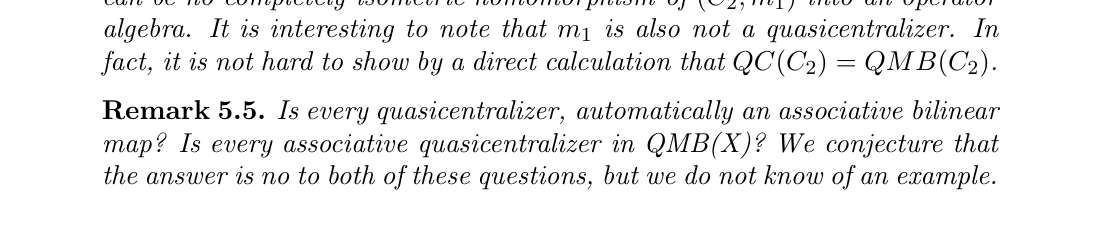
\includegraphics[width=0.93\textwidth]{figures/question_crop.png}
\end{center}

\textbf{Answer to the first question.} Yes: every quasicentralizer on every
operator space is automatically associative. Thus the conjectured answer to
the first question has the opposite sign. The second question is not needed
for this conclusion and is not claimed solved here.

\textbf{Definitions and canonical actions.} A bilinear map
$m:X\times X\to X$ is a quasicentralizer if there are completely bounded maps
\[
 \gamma:X\longrightarrow M_l(X),\qquad
 \psi:X\longrightarrow M_r(X)
\]
such that
\begin{equation}\label{eq:compat}
 m(x,y)=\gamma(x)y=x\psi(y)\qquad(x,y\in X).
\end{equation}
In the injective-envelope realization used in the source,
$X\subset I(X)$ is the $12$ corner of the linking $C^*$-algebra $I(S_X)$,
while $M_l(X)\subset I_{11}(X)$ and $M_r(X)\subset I_{22}(X)$. Consequently
their canonical actions obey
\begin{equation}\label{eq:commute}
 (a x)b=a(xb)\qquad
 (a\in M_l(X),\ x\in X,\ b\in M_r(X)),
\end{equation}
simply by associativity in $I(S_X)$.

\textbf{Proof intuition.} Use the right-multiplier formula for the outer
product in the left bracketing, and the left-multiplier formula for the outer
product in the right bracketing. The two expressions differ only by
parentheses in the linking algebra, so they coincide.

\begin{theorem}\label{thm:main}
Let $X$ be an operator space. Every quasicentralizer
$m:X\times X\to X$ is an associative bilinear map.
\end{theorem}

\begin{proof}
Choose $\gamma$ and $\psi$ as in \eqref{eq:compat}. For arbitrary
$x,y,z\in X$, apply respectively the right and left versions of
\eqref{eq:compat}, followed by \eqref{eq:commute}:
\begin{align*}
 m(m(x,y),z)
 &=m(x,y)\psi(z)
   =(\gamma(x)y)\psi(z)\\
 &=\gamma(x)(y\psi(z))
   =\gamma(x)m(y,z)
   =m(x,m(y,z)).
\end{align*}
Thus $m$ is associative.
\end{proof}

\textbf{Internal cross-check.} The same computation shows that $\gamma$ is
automatically the source's left quasihomomorphism. Indeed, for every $z\in X$,
\[
 \gamma(x)\gamma(y)z
 =\gamma(x)(y\psi(z))
 =(\gamma(x)y)\psi(z)
 =\gamma(m(x,y))z.
\]
Faithfulness of the canonical multiplier action gives
$\gamma(x)\gamma(y)=\gamma(m(x,y))$. Proposition 5.2 of the source then yields
associativity independently; the right-sided calculation is identical.

\textbf{The remaining second question.} Since associativity is automatic,
the second question becomes simply whether $QC(X)=QMB(X)$ for every operator
space. Eight focused upgrade attempts did not settle it. Exact rational
linear-algebra searches found equality for every connected matrix-unit
support through $3\times3$, all two-dimensional $0/1$ subspaces of
$M_{2,2}$, $M_{2,3}$, and $M_{3,2}$, and 400 deterministic random
three-dimensional $0/1$ subspaces of $M_{3,3}$. The general obstruction is
that compatibility makes the relevant multiplier maps completely bounded,
but does not visibly imply the special complete-contraction block estimates
which the source uses to produce one fixed middle quasimultiplier.

\textbf{Novelty and verification.} Exact-sentence, title, arXiv, and core-term
searches through 2026-08-13 found no later answer. The proof uses only the
source's definitions and canonical corner realization. Novelty confidence is
moderate pending specialist review. The accompanying verification report
checks every typing and corner multiplication and records the exact search
scope.

\textbf{Human-review recommendation.} Verify that the standard left and right
multiplier actions used in Definition 5.1 are the $11$- and $22$-corner
actions in $I(S_X)$. Equation \eqref{eq:commute} then makes the proof
immediate.

\begin{thebibliography}{9}
\bibitem{KP}
M. Kaneda and V. I. Paulsen,
\emph{Quasimultipliers of operator spaces},
J. Funct. Anal. 217 (2004), 347--365; arXiv:math/0312501.
\end{thebibliography}

\end{document}
